\documentclass[a4paper]{article}
\usepackage{anysize}
\marginsize{1cm}{1cm}{1cm}{1cm}

\usepackage{amssymb}
\usepackage{amsmath}
\usepackage[pdftex]{graphicx}
\usepackage{epsfig}
\usepackage{subfigure}
\usepackage{listings}
\lstset{language=haskell}
\lstset{commentstyle=\textit}
\lstset{mathescape=true}
\lstset{backgroundcolor=,rulecolor=}
\lstset{basicstyle=\ttfamily}
%\linespread{2.0}

\begin{document}

\title{\bf Monadic Object Encodings}

\author{Giuseppe Maggiore \quad Michele Bugliesi
 \\ Universit\`a Ca' Foscari Venezia
 \\ Dipartimento di Informatica 
 \\ \{maggiore,bugliesi\}@dsi.unive.it
}

\date{}
\maketitle

\begin{abstract}
In this paper we define a model for expressing highly generic
computations with objects in Haskell. Our objects manipulate
some abstract memory. We do so with a twofold objective:
\begin{itemize}
\item to be able to define various, different concrete 
implementations of our objects that implement different
behaviors such as transactional computations, reactive
programming, mutable programs, etc;
\item to be able to perform various kinds of static analysis 
on memory management and computations, thereby having 
type-safe dynamic memory management, type-safe reflection, 
and other similar opportunities.
\end{itemize}
\end{abstract}

\section{Introduction}
\label{sec:intro}
%----------------------------------------------------------------------------
%  intro.tex 
%----------------------------------------------------------------------------
Our goal is to define a set of operators that allow us to write
object-oriented programs in the Haskell language. Object orientation
can be used in conjunction with various paradigms, such as (these are
by no means the only possible fields of application): 
\begin{itemize}
\item mutable programs where the state inside each object can be
  transparently mutated by method calls and other kinds of
  manipulations 
\item concurrent programs where the inner state of each object does
  not belong to the same thread, process or even machine 
\item reactive programs where each stateful operation is recomputed
  whenever the values it depends from change 
\item transactional programs where each stateful operation is recorded
  and blocks of stateful operations can be undone 
\end{itemize}

We definitely wish to define our operators so that we can use anyone
of these paradigms for running our object-oriented programs. For this 
reason we define the object oriented operators abstractly, that is
inside type classes; we then proceed to give the concrete
implementations  that will allow us to actually run our code.

We also wish to make it simple to use our objects. One of the best
ways to make some abstraction simpler to code in the Haskell language
is to take advantage of monads and their syntactic sugar: we will try
to make use of monads whenever possible, and we will even require so
at the level of our typeclasses.

To make a working object oriented system in a type-safe and purely
functional language such as Haskell we are forced to define many  
type-level functions and predicates. A relevant side effect of this is
that all our entities are first class entities in the host language; 
this allows us to freely manipulate labels, method applications, and
so on, and even to design a type safe reflection system. 
 

\section{State}
\label{sec:state}
\subsection{Memory}
We start by defining a memory typeclass, which will define the basic environment for our computations. We model our memory after a stack for simplicity. The memory predicate is defined as follows:

\begin{lstlisting}
class Memory m where
  data Malloc :: * -> * -> *
  malloc :: m -> a -> Malloc a m
  free   :: Malloc a m -> m
  read   :: Malloc a m -> a
  write  :: a -> Malloc a m -> Malloc a m
\end{lstlisting}

Our memory supports type-safe allocation and deallocation 
thanks to two function, $malloc$ and $free$, and a type 
function $Malloc$ that defines the type of our memory 
to which a value of type $a$ is added. We also define accessors to $read$ and $write$ the elements of our memory.

\subsection{References and Statements}
We will never work directly with values, since what we are trying to accomplish requires that values are packed inside "smart" containers that are capable of doing more complex operations such as mutating a shared state, sending messages to other processes or tracking dependencies from other smart values to implement reactive updates. For this reason we will represent values in two different ways:
\begin{itemize}
\item as references whenever we wish to represent a pointer to some value inside the current memory
\item as statements whenever we wish to represent the result of arbitrary computations
\end{itemize}

References and statements are defined respectively with the $State$ predicate. Notice that we automatically associate
a reference to a state $st$ thanks to the type function 
$Ref$. We depart slightly from the standard representation 
of statements and stateful computations in that a statement in our system has different input and output types for the 
state, to allow the manipulation of the type of the memory
to be tracked.

\begin{lstlisting}
class State st where
  data Ref st :: * -> * -> *
  eval :: (Memory m) => Ref st m a -> st m m a
  (.=) :: (Memory m) => Ref st m a -> a -> st m m ()
  delete :: (Memory m) => st (Malloc a m) m ()
  new :: (Memory m) => a -> st m (Malloc a m) (Ref st (Malloc a m) a)
  (>>>=) :: (Memory m, Memory m', Memory m'') => st m m' a -> (a -> st m' m'' b) -> st m m'' b
  (>>>) :: (Memory m, Memory m', Memory m'') => st m m' a -> st m' m'' b -> st m m'' a
\end{lstlisting}

The $st$ functor applied to the memory $m$ twice is required by this definition to be a monad; thanks to this we can use our operators on references taking advantage of the syntactic sugar that Haskell offers, obtaining code that is much more intuitive to a programmer used to traditional object oriented languages.

We give an evaluation operator that evaluates (dereferences) 
a reference into a corresponding statement and an assignment 
operator to assign a reference a constant value.

The $new$ and $delete$ operators respectively add and remove a single value from our memory.

To concatenate regular statements and state transition statements we define the $(>>+)$ operator, which is a generalized binding operator: $(>>=)$ is defined in terms of $(>>+)$ for the state monad, since $(>>=)$ simply imposes the constraint that both parameters of $st$ are the same.

In our examples, we will use syntactic sugar that is not available in Haskell to make using the $(>>+)$ operator transparent; we call this the $do+$ notation.

We also define a shortcut for in-place modification of a 
reference:
\begin{lstlisting}
(*=) :: (State st,Memory s, Monad (st s s)) => Ref st s a -> (a->a) -> st s s ()
ref *= f = do v <- eval ref
              ref .= (f v)
\end{lstlisting}
 

\section{Records}
\label{sec:records}
\section{Records}
We build mutable records in addition to our preceding operators. A record simply needs labels and the possiblity to (mutably) select a
field from a record. Since we want to ensure mutability, we want our selection operator to take as input a reference to our record and
to return as output a reference to the selected field; references can be assigned and evaluated (thanks to the $:=$, $*=$ and $eval$
operators) and this is what does guarantee mutability:

\begin{lstlisting}
class (State st m) => Record r st m where
  data Label st r :: * -> *
  (<==) :: (Ref st) m r -> Label st r a -> (Ref st) m a\end{lstlisting}
 

\section{Mutable Implementation}
\label{sec:mutable_implementation}
\section{Mutable Implementation}
We now give the implementation of the operators seen until now with a simple mutable state.

We define our state as that of the state monad (that is a statement that evaluates to a value of type $a$ in a state of type $s$ has the same type of its denotational semantics):
\begin{lstlisting}
data St s s' a = St(s->(a,s'))
\end{lstlisting}

References will be based on the state since a reference must be easily convertible into statements, one for evaluating the reference and one for assigning it:
\begin{lstlisting}
type Get s a = St s s a
type Set s a = a -> St s s ()
\end{lstlisting}

We now need to represent the state (our memory). The simplest implementation of a typed memory is based on heterogeneous lists. A heterogeneous list is build based on two type constructors:
\begin{lstlisting}
data Nil = Nil deriving (Show)
\end{lstlisting}

Since heterogeneous lists do not have a single type, we characterize all heterogeneous lists with an appropriate predicate:
\begin{lstlisting}
class HList l
instance HList Nil
instance HList tl => HList (Malloc h tl)

infixr `Malloc`
\end{lstlisting}

We access heterogeneous lists by index. To ensure type safety we define type-level integers, encoded as Church Numerals:
\begin{lstlisting}
data Z = Z
data S n = S n

class CNum n
instance CNum Z
instance CNum n => CNum (S n)
\end{lstlisting}

We can now read the length of a heterogeneous list, as well as get the type of an arbitrary element of the list:

\begin{lstlisting}
type family HLength l :: *
type instance HLength Nil = Z
type instance HLength (Malloc h tl) = S (HLength tl)

type family HAt l n :: *
type instance HAt (Malloc h tl) Z = h
type instance HAt (Malloc h tl) (S n) = HAt tl n
\end{lstlisting}

We will need a way to manipulate the values of a heterogeneous list. For this reason we define a lookup predicate:
\begin{lstlisting}
class (HList l, CNum n) => HLookup l n where
  lookup :: l -> n -> HAt l n
  update :: l -> n -> HAt l n -> l

instance (HList tl) => HLookup (Malloc h tl) Z where
  lookup (Malloc h tl) _ = h
  update (Malloc h tl) _ h' = (Malloc h' tl)

instance (HList tl, CNum n, HLookup tl n) => HLookup (Malloc h tl) (S n) where
  lookup (Malloc _ tl) _ = lookup tl (undefined::n)
  update (Malloc h tl) _ v' = (Malloc h (update tl (undefined::n) v'))
\end{lstlisting}

Now we have all that we need to instance our memory, reference and state predicates.

We begin by instancing the $Memory$ predicate, since all heterogeneous lists are memory and as such can be used:
\begin{lstlisting}
instance (HList m) => Memory m where
  data Malloc a m = Malloc a m deriving (Show)
  malloc m a = Malloc a m
  free (Malloc h tl) = tl
  read   (Malloc h tl) = h
  write  h' (Malloc h tl) = Malloc h' tl
\end{lstlisting}

We instance the $Monad$ class with the $St$ type (as in the state monad):
\begin{lstlisting}
instance Monad (St s s) where
  return x = St(\s -> (x,s))
  (St st) >>= k = St(\s -> 
                          let (res,s') = st s 
                              (St k') = k res
                          in k' s')
\end{lstlisting}

We also define a way to evaluate a statement and ignoring the resulting state:
\begin{lstlisting}
runSt :: St s s' a -> s -> a
runSt (St st) s = fst (st s)
\end{lstlisting}

Now that $Monad (St s)$ is instanced we can instance the $State$ predicate for our references and state:
\begin{lstlisting}
instance (HList m, n~HLength m) => State St m where
  data Ref St m a = StRef (Get m a) (Set m a)
  eval (StRef get set) = get
  (StRef get set) .= v = set v
  delete = St(\s -> ((), free s))
  new v = let new_ref = StRef (St (\s -> (read s, s)))
                              (\v' -> St(\s -> ((), write v' s)))
          in St (\s -> (new_ref, malloc s v))
  (St st) >>+ k = St(\s -> 
                            let (res,s') = st s 
                                (St k') = k res
                            in k' s')
\end{lstlisting}

Thanks to this last instance we can now give a first working example of usage of our references with mutable state:
\begin{lstlisting}
ex1 = do+ i <- new 10
          i *= (+2)
          eval i

res1 :: Int
res1 = runSt ex1 Nil
\end{lstlisting}

The result, as expected, is $res1=12$.

We complete the implementation of our system so far by adding records. We use as records heterogeneous lists to which we access via labels. A label is defined with a getter and a setter (similar to those found in the $Ref$ constructor) as:
\begin{lstlisting}
\end{lstlisting}

We can instance the $Record$ predicate:
\begin{lstlisting}
instance (HList m, HList r) => Record r St m where
  data Label St r a = StLabel (r->a) (r->a->r)
  StRef get set <== StLabel read write =
    StRef(do r <- get
             return (read r))
         (\v'-> do r <- get
                   set (write r v'))
\end{lstlisting}

To more easily manipulate records we define a function for building labels from $CNum$s:
\begin{lstlisting}
labelAt :: forall l n . (HList l, CNum n, HLookup l n) => n -> Label St l (HAt l n)
labelAt _ = StLabel (\l -> lookup l (undefined::n)) 
                    (\l -> \v -> update l (undefined::n) v)
\end{lstlisting}

We can now give a second example that shows how records can be manipulated:
\begin{lstlisting}
type Person = String `Malloc` String `Malloc` Int `Malloc` Nil
first :: Label St Person String
first = labelAt Z
last :: Label St Person String
last = labelAt (S Z)
age :: Label St Person Int
age = labelAt (S (S Z))

mk_person :: String -> String -> Int -> Person
mk_person f l a = (f `Malloc` l `Malloc` a `Malloc` Nil)

ex2 = do+ p <- new (mk_person "John" "Smith" 27) :: Ref (New Nil Person) Person
          (p <= last) *= (++ " Jr.")
          (p <= age) := 25
          eval p)

res2 = runSt ex2 Nil
\end{lstlisting}
The result is, as expected, $"John"\ 'Cons'\ "Smith Jr."\ 'Cons'\ 25\ 'Cons'\ Nil$.

We give one last example that does not work even though at a first glance we would expect it to. This example is used to introduce the next session:
\begin{lstlisting}
ex3_wrong :: St Nil (Malloc (Malloc Nil Int) String) Unit
ex3_wrong = do+ i <- new 10 :: Ref (New Nil Int) Int
                s <- new "Hello" :: Ref (New (New Nil Int) String) String
                i *= (+2)
                s *= (++" World")
                return ())
\end{lstlisting}

This example does not even compile because:
\begin{lstlisting}
i *= (+2) :: St (New Nil Int) ()
\end{lstlisting}

while
\begin{lstlisting}
s *= (++" World") :: St (New (New Nil Int) String) ()
\end{lstlisting}

but the state monad cannot accept a state that varies between statements. It is of course worthy of notice that the above sample, though as it is does not compile, is definitely not nonsensical. Whenever we have a larger state such as 
\begin{lstlisting}
New (New Nil Int) String
\end{lstlisting}

we expect to be able to work with references that expect a smaller state, such as
\begin{lstlisting}
New Nil Int
\end{lstlisting}

since all that is needed for them to work is contained in the larger state, and through appropriate conversion both reading and writing on the smaller state can be performed on the larger state. The notion we will use to fix this problem happens to be that of coercive subtyping.
 

\section{Coercive Subtyping}
\label{sec:subtyping}
\subsection{Coercible}
We now discuss a possible solution to the problems encountered when defining the sample $ex3_wrong$. We give a predicate that expresses the relation of coercive subtyping:
\begin{lstlisting}
class Coercible a b where
  coerce :: a -> b
\end{lstlisting}

\subsection{Coercion for References}
We wish to instance the coercion predicate to references. References are:
\begin{itemize}
\item covariant in the referenced type
\item contravariant in the state type
\end{itemize}
This happens because a reference to some $a$ can be used whenever a reference to an $a$ such that $a \le a'$ is expected, and also (as seen in the third example above), a reference that works on a state $s'$ can be used whenever a state $s$ such that $s \le s'$ is available. Of course, the fact that references express not only reading values and states but also writing will make this operation relatively tricky.

At the moment we will only focus on expressing the coercion relation for the state of the reference; the coercion relation for the value of the reference will be discussed together with inheritance.

The kind of operation that we wish to perform when coercing a reference to work on a larger memory is summarized in Figure \ref{fig:ref_coerce}. Whenever we wish to perform some operation on a reference to the smaller memory, we will:
\begin{itemize}
\item take only the first part of the (larger) input memory 
\item perform the operation on the obtained smaller memory through the original reference we have coerced
\item replace the first part of the (larger) input memory with the (smaller) modified memory
\end{itemize}

\begin{figure}[h]
\centerline{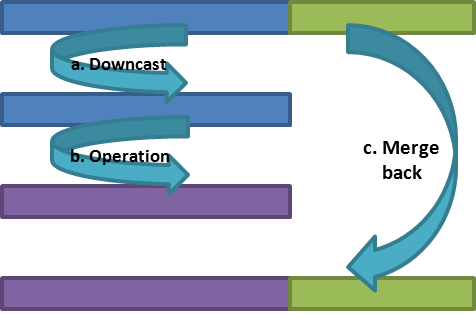
\psfig{file=heap_upcasting.png,height=5cm}} \caption{Coercing references.\label{fig:ref_coerce}}
\end{figure}

We instance the coercion predicate for references to perform a single step of coercion, that is for the case when we have a reference to a memory $tl$ and we want to use it where we expect a memory $Cons\ h\ tl$:
\begin{lstlisting}
instance HList tl => Coercible (Ref St tl a) (Ref St (Malloc h tl) a) where
  coerce ref =
    StRef (St(\(Malloc h tl) ->
                          let (res, tl') = get ref tl
                          in (res, h `Malloc` tl')))
          (\v -> St(\(Malloc h tl) -> 
            let ((),tl') = set ref tl v
            in ((),h `Malloc` tl')))
    where get (StRef (St g) _) = g
          set (StRef _ s) = \st -> \v -> 
                                         let (St s') = s v
                                         in s' st
\end{lstlisting}

Now we can finally rewrite the example above to make use of our new coercion operator:
\begin{lstlisting}
ex3 :: forall m0 m1 m2 st . (HList m0, State st, m1 ~ Malloc Int m0, m2 ~ Malloc String m1, Monad (st m2 m2),
                             Coercible (Ref st m1 Int) (Ref st m2 Int)) => st m0 m2 String
ex3 = do+ i <- new 10
          s <- new "Hello"
          ((coerce i) :: Ref St (String `Malloc` Int `Malloc` Nil) Int) *= (+2)
          s *= (++ " World")
          eval s

res3 = runSt ex3 Nil
\end{lstlisting}
 

\section{Objects}
\label{sec:objects}
\section{Objects}
We now start with the characterization of objects in our system. The $Object$ predicate says that an object will be a record which supports methods and inheritance; of course all the object operators are expected to work in conjunction with the rest of the system. Since objects will reference themselves, to avoid recursive type definitions we give a predicate that allows us to freely add or remove some constructor from an object:
\begin{lstlisting}
class Recursive o where
  type Rec o :: *
  to :: o -> Rec o
  from :: Rec o -> o
\end{lstlisting}

An object is required to support the $Recursive$ predicate:
\begin{lstlisting}
class (Record o st s, Recursive o, ro~Rec o) => Object o st s where
  type Base o :: *
  get_base :: Ref st s o -> Ref st s (Base o)

  type Method ro st :: * -> * -> *
  (<=|) :: Ref st s r -> Label r (Method ro st a b) -> a -> st s b
\end{lstlisting}

With respect to inheritance, it looks clear how we can instance coercion to take advantage (and make access more uniform) of the $base$ operations:
\begin{lstlisting}
instance Object o st s => Coercible (Ref st s o) (Ref st s (Base o)) where
  coerce = get_base
\end{lstlisting}

We also add a further predicate that characterizes inheritance:
\begin{lstlisting}
class Inherits a b

instance (Object o st s) => Inherits o (Base o)
\end{lstlisting}

Notice that methods are defined with a different operator than the selection operator for records. This can be addressed as follows: we define a new predicate for selecting something from a reference through a label:
\begin{lstlisting}
class Selectable st t s a where
  type Selection s t a :: *
  (<=) :: Ref st s t -> Label t a -> Selection s t a
\end{lstlisting}

We instance this predicate twice, one for field selection and one for method selection. Before doing so, though, we must be careful to disambiguate the last parameter in the record definition. For this purpose we add a $Field$ type function that represents a placeholder type that will distinguish fields from methods and inherited types:
\begin{lstlisting}
class (RefSt st s) => Record r st s where
  type Label r :: * -> *
  type FieldSlot a :: *
  (<==) :: Ref st s r -> Label r (FieldSlot a) -> Ref st s a
\end{lstlisting}

In the case of simple mutable records we can easily add a trivial constructor for $FieldSlot$ such as:
\begin{lstlisting}
data Field a = Field a
\end{lstlisting}

Now we can instance the selection predicate:
\begin{lstlisting}
instance Record st r s => Selectable st r s (FieldSlot a) where
  type Selection s r (Field a) = Ref st s a
  (<=) = (<==)

instance (Object st o s, ro~Rec o) => Selectable st o s (Method ro a b) where
  type Selection s o (Method ro a b) = a -> st s b
  (<=) = (<=|)
\end{lstlisting}

The final operation we wish to support is that of selecting a method or a field directly from any of the inherited classes of an object without explicit coercions:
\begin{lstlisting}
instance (Object st o s, bo~Base o, Selectable st bo s a) => Selectable st o s a where
  type Selection s o a = Selection s bo a
  (<=) = get_base . (<=)
\end{lstlisting} 

\section{Mutable Objects}
\label{sec:mutable_objects}
We now implement mutable objects. We start with inheritance:
\begin{lstlisting}
instance (Recursive o, Record o St) => Object o St where
  data Method St ro a b = StMethod(ro -> a -> (b,ro))
  self_ref <=| (StLabel read write) = 
             \x -> do self <- eval self_ref
                      let (StMethod m) = read self
                          (res,self' :: Rec o) = m (to self) x
                      self_ref .= (from self')
                      return res
  mk_method m = StMethod(\this -> \args -> let (St res_st) = m id_ref args
                                               (res,this' :: o) = res_st ((from this) :: o)
                                           in (res,((to this') :: Rec o)))
                where id_ref = StRef (St (\s -> (s,s))) (\s' -> (St (\s -> ((),s'))))
\end{lstlisting}
In our mutable encoding the first field of the object must be either the value of the inherited value or unit when the object does not inherit anything.

Methods enjoy the same implementation in both cases, so we just give one:
\begin{lstlisting}
instance (Object o St, o ~ (Malloc (Inherit b) so)) => Inherits o b St where
  data Inherit a = StInherit a
  get_base self_ref =   StRef(do ((StInherit base) `Malloc` tl) <- eval self_ref
                                 return base)
                             (\base' -> do (_ `Malloc` tl) <- eval self_ref
                                           self_ref .= ((StInherit base') `Malloc` tl)
                                           return ())
\end{lstlisting}

It can prove very useful to take advantage of our existing infrastructure to create methods from references and statements, so that the user of our system will not be forced to define methods by explicitly tracking mutations to the value of $this$; for this reason we add a function to the $Object$ predicate that converts a method from reference to state into our format (the implementation here is the same for both instances of $Object$, so we provide only one:
\begin{lstlisting}
instance (Inherits o b st, Memory s) => Coercible (Ref st s o) (Ref st s b) where
  coerce = get_base
         in res_st this)
\end{lstlisting} 

\section{Sample: Vectors}
\label{sec:vectors}
We now implement a simple example that shows how we can define a system of mutable vectors.

We begin by defining a 2d vector ($Vector2$) with two methods and a 3d vector ($Vector3$) with two other methods and which inherits the 2d vector:
\begin{lstlisting}
type Vector2Def k = Field St Float `Malloc` Field St Float `Malloc` Method St k () () `Malloc` Method St k () Float `Malloc` Nil
data RecVector2 = RecVector2 (Vector2Def RecVector2)
type Vector2 = Vector2Def RecVector2
instance Recursive Vector2 where
  type Rec Vector2 = RecVector2
  to = RecVector2
  from (RecVector2 v) = v
x :: Label St Vector2 (Field St Float)
x = labelAt Z
y :: Label St Vector2 (Field St Float)
y = labelAt (S Z)
norm2 :: Label St Vector2 (Method St (Rec Vector2) () ())
norm2 = labelAt (S (S Z))
len2 :: Label St Vector2 (Method St (Rec Vector2) () Float)
len2 = labelAt (S (S (S Z)))

mk_vector2 :: Float -> Float -> Vector2
mk_vector2 xv yv = (StField xv) `Malloc` (StField yv) `Malloc` norm `Malloc` len `Malloc` Nil
                    where norm = mk_method (\this -> \() -> do l <- (this <= len2) ()
                                                               (this <= x) *= (/ l)
                                                               (this <= y) *= (/ l))
                          len = mk_method (\this -> \() -> do xv <- eval (this <= x)
                                                              yv <- eval (this <= y)
                                                              return (sqrt(xv * xv + yv * yv)))

type Vector3Def k = Inherit Vector2 `Malloc` Field St Float `Malloc` Method St k () () `Malloc` Method St k () Float `Malloc` Nil
data RecVector3 = RecVector3 (Vector3Def RecVector3)
type Vector3 = Vector3Def RecVector3
instance Recursive Vector3 where
  type Rec Vector3 = RecVector3
  to = RecVector3
  from (RecVector3 v) = v
z :: Label St Vector3 (Field St Float)
z = labelAt (S Z)
norm3 :: Label St Vector3 (Method St (Rec Vector3) () ())
norm3 = labelAt (S (S Z))
len3 :: Label St Vector3 (Method St (Rec Vector3) () Float)
len3 = labelAt (S (S (S Z)))

mk_vector3 :: Float -> Float -> Float -> Vector3
mk_vector3 xv yv zv = StInherit (mk_vector2 xv yv) `Malloc` StField zv `Malloc` norm `Malloc` len `Malloc` Nil
                      where norm = mk_method (\this -> \() -> do l <- (this <= len3) ()
                                                                 ((get_base this) <= x) *= (/l)
                                                                 ((get_base this) <= y) *= (/l)
                                                                 (this <= z) *= (/l)) 
                            len = mk_method (\this -> \() -> do xv <- eval ((get_base this) <= x)
                                                                yv <- eval ((get_base this) <= y)
                                                                zv <- eval (this <= z)
                                                                return (sqrt(xv * xv + yv * yv + zv * zv)))

ex4 :: forall mem . mem ~ (Vector3 `Malloc` Nil) => St Nil Nil Bool
ex4 = do+ v <- new (mk_vector3 0.0 2.0 (-1.0))
          xv <- eval ((get_base v) <= x)
          let v' = coerce v :: Ref St mem Vector2
          xv' <- eval (v' <= x)
          (v' <= norm2)()
          (v <= norm3)()
          return (xv == xv')
          delete

res4 :: Bool
res4 = runSt ex4 Nil
\end{lstlisting}

where we expect that $res=True$. Notice how select labels that are defined for a 2d vector on an instance of a 3d vector, and how we access the same label on the value of $base$ obtained through coercion on the 3d vector.
 

\section{Alternate Implementations}
\label{sec:alternate}
In the following sections we give alternate implementations of our system. We do so in order to exploit its flexibility by showing how the same primitives allow us to define very different execution models:
\begin{itemize}
\item A transactional model
\item A concurrent/distributed model
\item A reactive model
\end{itemize}

Each model is characterized by a predicate that expresses some requirements on its state, reference or stack types so as to allow different implementations of the same model (for example to experiment with faster algorithms, etc).

The predicate for the transactional model simply states that there must be three methods for opening, closing and undoing transactions. Notice that transactions might also be used for implementing undo buffers in a very simple and clean way:
\begin{lstlisting}
class Transactional st where
  beginT :: st s ()
  commitT :: st s ()
  abortT :: st s ()
\end{lstlisting}

The predicate for concurrency requires a method for forking computations:
\begin{lstlisting}
class Concurrent st where
  fork :: (st s (), st s ()) -> st s ()
\end{lstlisting}

The reactive model has no specific requirements, and is simply an alternate instantiation of the object system typeclasses.

In addition to these three implementations, we will discuss a system for reflection on objects. Reflective objects will validate a predicate ($ReflectiveObject$) which allows to obtain the labels that respect certain conditions; being labels first class objects, they will then be passed around and used freely for selection on objects of the appropriate type:
\begin{lstlisting}
class (Object o ref st s, ro~Rec o) => ReflectiveObject o ref st s where
  get_fields :: [Label o (Field a)]
  get_methods :: [Label o (Method ro a b)]
\end{lstlisting}
 

\end{document}
